\documentclass{article}
\usepackage{arxiv}
\usepackage[utf8]{inputenc}
\usepackage[T1]{fontenc}
\usepackage{xcolor}
\definecolor{cblue}{HTML}{2A78D6}\definecolor{corange}{HTML}{EB6834}\definecolor{cviolet}{HTML}{4A3AA7}
\definecolor{cgray}{HTML}{52514E}\definecolor{clight}{HTML}{F2F1EC}\definecolor{cred}{HTML}{E34948}
\usepackage{hyperref}
\hypersetup{colorlinks=true,linkcolor=cblue,citecolor=cblue,urlcolor=cblue}
\usepackage{url}
\usepackage{booktabs}
\usepackage{amsfonts,amsmath,amssymb}
\usepackage{microtype}
\usepackage{graphicx}
\usepackage{natbib}
\usepackage{tikz}
\usetikzlibrary{positioning,arrows.meta,fit,backgrounds,calc}
\usepackage{enumitem}
\usepackage{caption}
\captionsetup{font=small}
\newcommand{\dauc}{$\Delta$AUC}

\title{Typed Is Not Always Better: Jev-Style Decision Models for Medical Vision--Language Tasks}

\author{
  Author Name(s) \\
  Affiliation \\
  \texttt{email@domain} \\
}
\renewcommand{\headeright}{Preprint}
\renewcommand{\undertitle}{Preprint}
\renewcommand{\shorttitle}{Typed Is Not Always Better}

\begin{document}
\maketitle

\begin{abstract}
Medical vision--language models can answer checklist-style diagnostic questions, but generated answers must be parsed and carry no probability for each admissible option. Typed decision models (TDMs) such as Jev return one probability per caller-defined option, and we develop a vision interface that connects the native Qwen3.5 encoder to Kev, an open TDM. The image is encoded once as a shared state, and each clinical criterion is answered in an isolated branch whose options are scored by a pointer head. On text inputs, the interface reproduces the released model exactly. We further examine decision-oriented pretraining by fine-tuning the same architecture either from Kev's weights or from the base model. We evaluate typed and label-probability readouts, linear probes and fine-tuned models on the official test splits of Derm7pt, SLAKE, VQA-RAD and PubMedQA. Built on Qwen3.5-0.8B, the fine-tuned typed model achieves mean AUCs of 0.851 on the seven Derm7pt criteria and 0.981 on SLAKE, the highest among the compared models, and the typed readout exceeds label probabilities on the multi-option dermoscopic criteria but not on binary radiology questions. Initialization from Kev adds 0.012 AUC on Derm7pt and reduces the AUC loss under displaced option names from 0.040 to 0.011 on Derm7pt validation; on VQA-RAD, none of the Kev-initialized runs collapsed, whereas one base-initialized run did. On PubMedQA, the hosted Jev reaches the highest macro-F1 (0.636) but a higher calibration error than open 4B-scale models. These results show how typed readouts and decision-oriented pretraining can support robust medical decisions, provided that calibration is verified on in-domain data.
\end{abstract}

\keywords{Typed decision models \and Medical vision--language models \and Calibration \and Robustness \and Dermoscopy}

%==========================================================================
\section{Introduction}
%==========================================================================
Medical vision--language models are extending image analysis from fixed-label prediction toward question-conditioned interpretation. General-purpose models accept images at arbitrary resolution through a shared language interface~\citep{wang2024qwen2vl,qwen35}, and biomedical assistants such as LLaVA-Med answer visual questions about radiology and pathology images~\citep{li2023llavamed}. Benchmarks such as VQA-RAD and SLAKE evaluate these models on clinically posed questions~\citep{lau2018vqarad,liu2021slake}. Many of these questions are decisions over a small set of clinically defined options: whether a finding is present, or which pattern describes a lesion. This setting raises a central question for clinical decision support: how should a model expose its decision over a fixed set of clinically defined options?

Generated text is an indirect answer to that question. The answer must be parsed from free text, may fall outside the admissible set, and carries no probability that a downstream rule can threshold. Reading the probability of each answer label from the next-token distribution avoids parsing, but it is sensitive to the surface form of the label and to label priors~\citep{holtzman2021surface,zhao2021calibrate}. It also depends on how a model binds option symbols to option content and on the order in which options are listed~\citep{robinson2023mcq,pezeshkpour2023order,zheng2024mcq}. These observations motivate an interface in which each admissible option, together with its definition, receives an explicit probability.

Typed decision models (TDMs) provide such an interface. Jev, a hosted TDM, returns a distribution over the options of yes/no, multiple-choice and ordinal questions and is described by its developer as trained for calibrated decisions~\citep{typesafe2026jev,typesafe2026blog}. Open reconstructions include Kev, which adds a pointer head to a Qwen3.5 backbone, and reflex, which reads option probabilities from a frozen model~\citep{palmer2026kev,raghavan2026reflex}. Visual variants have been studied on natural images~\citep{yu2026visualjev,zhou2026pixeljev}, and a review of the early literature found that most evaluations omit a label-probability control and that calibration depends on the workload~\citep{audit2026tdm}. Our focus is how typed readouts behave when the state is a medical image and every option carries a clinical definition.

The first consideration is the readout itself. A typed readout scores each option span against a decision token, so the score can depend on the full text of the option. A label-probability readout scores a label token, so it depends on how the model has bound that label to the option content. When questions have more than two options and options are defined by clinical descriptions, the two readouts may therefore differ, whereas for yes/no questions they may coincide. We therefore compare both readouts on models of the same size and on the same questions.

The second consideration is what decision-oriented pretraining contributes once a model is fine-tuned on medical data. Kev's released weights were trained on text decision tasks with varied option orders and distractor options~\citep{palmer2026kev}. Such pretraining might raise accuracy, stabilize training on small datasets, or reduce the tendency of TDMs to follow option names rather than option definitions~\citep{sun2026typesafe}. Each of these effects would matter in practice, but accuracy alone cannot distinguish them. A fair test therefore requires fine-tuning from decision-trained and from newly initialized heads under identical conditions, together with diagnostics of calibration and of sensitivity to option wording.

We develop a vision interface for Kev built around these two comparisons. Kev loads only the text part of its natively multimodal backbone, so we take the vision encoder from the same checkpoint and insert its visual tokens into the state segment. The image is encoded once, and each question forms an isolated branch that ends in a decision token. A pointer head scores every option span against that token and returns a distribution over options. On text inputs, the interface reproduces the outputs of the released model, so any change on images can be attributed to the visual state.

The second component is decision-oriented initialization. We fine-tune the low-rank adapters and the pointer head of the same backbone either from Kev's weights or from a new initialization, while the vision encoder, the data, the augmentations and the schedule remain fixed. The comparison does not assume that decision-oriented pretraining helps accuracy; it measures accuracy, training stability and reliance on option names separately. Model selection is restricted to the final training epoch, so no comparison depends on checkpoint choice.

We evaluate the interface on dermoscopic checklist criteria from Derm7pt, closed radiology questions from SLAKE and VQA-RAD, and biomedical question answering from PubMedQA~\citep{kawahara2019derm7pt,jin2019pubmedqa}. Each comparison isolates one factor: typed against label-probability readouts on backbones of the same size, fine-tuned models against linear probes on the same frozen encoder, and decision-oriented against new initialization under the same schedule. All results use the official test splits, decision rules were fixed before each test set was evaluated, and the hosted Jev is evaluated on the text benchmark it supports.

The main contributions are summarized as follows:
\begin{itemize}[leftmargin=*,itemsep=1pt,topsep=2pt]
  \item We introduce a vision interface for an open typed decision model that inserts native visual tokens into the decision state and reproduces the released model exactly on text inputs.
  \item We develop a controlled protocol that pairs typed with label-probability readouts and decision-oriented with new initialization, and that measures calibration and sensitivity to option wording alongside accuracy.
  \item We evaluate the approach on four public benchmarks, where the fine-tuned typed model obtains the highest AUC among the compared models on dermoscopic criteria and SLAKE, decision-oriented pretraining mainly improves robustness to option wording, and the hosted model is less well calibrated than open models on PubMedQA.
\end{itemize}

%==========================================================================
\section{Related Work}
%==========================================================================
\subsection{Typed Decision Models and Decision Interfaces}
Jev introduced a hosted interface in which a caller submits a state and typed questions and receives a distribution over each question's options~\citep{typesafe2026jev,typesafe2026blog}. Kev reconstructs this interface with low-rank adaptation~\citep{hu2022lora} of a Qwen3.5 backbone and a pointer head over option spans, while reflex reads option probabilities from a frozen model and averages over option orders~\citep{palmer2026kev,raghavan2026reflex}. Visual Jev and PixelJev adapt small vision--language models to typed visual choices on natural images and read decisions from the language-model head~\citep{yu2026visualjev,zhou2026pixeljev}. These systems establish the interface; our interest is in its behavior on medical images with clinically defined options.

Evaluations of these systems have appeared alongside them. A review of the early literature reports that most papers omit a label-probability readout of the same backbone and recommends controls for option names, repeated requests and calibration~\citep{audit2026tdm}. Individual studies show that TDMs can follow an option's name rather than the rubric attached to it~\citep{sun2026typesafe}, that Jev's probabilities omit an explicit ``I don't know'' mass~\citep{porcedda2026sys1cal}, and that Jev can serve as a selective judge or check radiology reports~\citep{li2026jevjudge,huang2026radjev}. These studies examine text workflows, rather than image-based decisions with fine-tuning and matched initializations.

\subsection{Option Scoring and Calibration in Language Models}
Scoring answer labels with a language model is a standard way to obtain zero-shot classifiers. Holtzman et al. show that probability mass is split across surface forms of the same answer~\citep{holtzman2021surface}, and contextual calibration corrects label priors estimated from content-free inputs~\citep{zhao2021calibrate}. Robinson and Wingate relate multiple-choice accuracy to a model's ability to bind option symbols to content~\citep{robinson2023mcq}, and several studies document sensitivity to option order~\citep{pezeshkpour2023order,zheng2024mcq}. These results concern generative readouts; our comparison places a trained typed readout next to them on identical questions.

Calibration of neural networks is commonly measured by expected calibration error~\citep{naeini2015ece} and corrected by temperature scaling~\citep{guo2017calibration}. Pre-trained transformers can be well calibrated in domain but less so under distribution shift~\citep{desai2020calibration}, whereas generative language models answering questions are often poorly calibrated~\citep{jiang2021calibration}. Larger models assess their own correctness more reliably~\citep{kadavath2022know}, and verbalized confidences have been proposed for models tuned with human feedback~\citep{tian2023justask}. Our distinction lies in measuring the calibration of typed readouts, including a hosted model marketed for calibrated decisions, on medical benchmarks.

\subsection{Medical Vision--Language Models and Concept-Based Diagnosis}
Medical visual question answering benchmarks such as VQA-RAD and SLAKE contain closed and open questions about radiology images~\citep{lau2018vqarad,liu2021slake}, and instruction-tuned biomedical models are commonly evaluated on them~\citep{li2023llavamed}. PubMedQA poses yes/no/maybe questions over research abstracts~\citep{jin2019pubmedqa}. BiomedCLIP provides image--text representations pretrained on biomedical figure--caption pairs~\citep{zhang2023biomedclip}. These resources evaluate answer accuracy, rather than the form in which a decision is returned.

Concept bottleneck models predict a label through human-interpretable concepts~\citep{koh2020cbm}. For skin lesions, dermoscopic checklist criteria provide such concepts: Derm7pt supplies per-lesion expert labels for the seven-point checklist~\citep{kawahara2019derm7pt}, and SkinCon supplies dense concept annotations for clinical images~\citep{daneshjou2022skincon}. Checklist criteria are naturally typed questions with defined options. We therefore use them to study typed readouts, and the next section describes the interface.

%==========================================================================
\section{Method}
%==========================================================================
\begin{figure}[t]
\centering
\resizebox{\linewidth}{!}{%
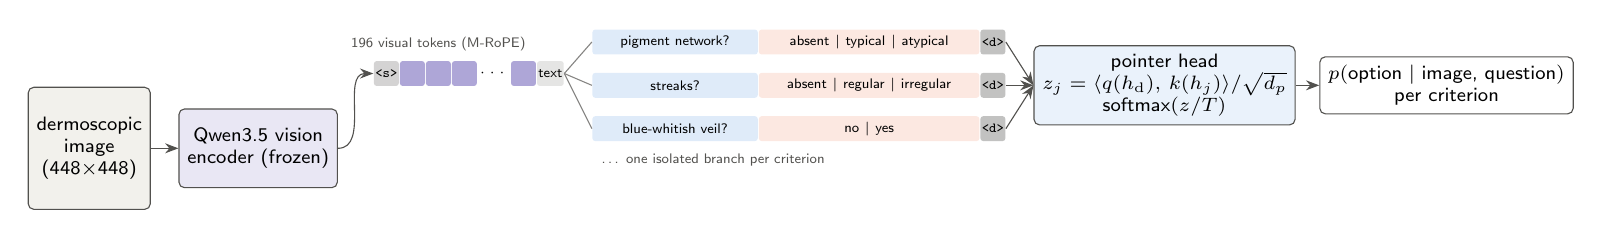
\begin{tikzpicture}[font=\sffamily\scriptsize, >=Stealth,
  box/.style={draw=cgray, rounded corners=2pt, fill=white, inner sep=3pt, align=center},
  tok/.style={draw=none, rounded corners=1pt, minimum height=9pt, minimum width=9pt, inner sep=0.5pt, font=\sffamily\tiny}]
  \node[box, minimum width=1.55cm, minimum height=1.55cm, fill=clight] (img) at (0,0) {dermoscopic\\image\\(448$\times$448)};
  \node[box, right=0.35cm of img, minimum height=1.0cm, fill=cviolet!12] (vit) {Qwen3.5 vision\\encoder (frozen)};
  \draw[->, cgray] (img) -- (vit);
  \node[tok, fill=cgray!25, right=0.45cm of vit, yshift=0.95cm] (s0) {\texttt{<s>}};
  \foreach \i/\c in {1/cviolet!45,2/cviolet!45,3/cviolet!45}{\node[tok, fill=\c, right=0pt of s\the\numexpr\i-1\relax] (s\i) {};}
  \node[tok, right=0pt of s3] (sdots) {$\cdots$};
  \node[tok, fill=cviolet!45, right=0pt of sdots] (s4) {};
  \node[tok, fill=cgray!15, right=0pt of s4] (s5) {text};
  \node[above=0pt of s2, font=\sffamily\tiny, cgray] {196 visual tokens (M-RoPE)};
  \draw[->, cgray] (vit.east) to[out=0,in=180] (s0.west);
  \foreach \k/\q/\o in {1/{pigment network?}/{absent $\mid$ typical $\mid$ atypical},2/{streaks?}/{absent $\mid$ regular $\mid$ irregular},3/{blue-whitish veil?}/{no $\mid$ yes}}{
    \node[tok, fill=cblue!15, minimum width=2.1cm, anchor=west] (q\k) at ($(s5.east)+(0.35cm, 0.95cm-\k*0.55cm)$) {\q};
    \node[tok, fill=corange!15, minimum width=2.8cm, right=0pt of q\k] (o\k) {\o};
    \node[tok, fill=cgray!35, right=0pt of o\k] (d\k) {\texttt{<d>}};
    \draw[cgray!70] (s5.east) -- (q\k.west);
  }
  \node[font=\sffamily\tiny, cgray, below=1pt of q3.south west, anchor=north west] {\ldots\ one isolated branch per criterion};
  \node[box, right=0.35cm of d2, fill=cblue!10] (ph) {pointer head\\$z_j = \langle q(h_{\mathrm{d}}),\, k(h_j)\rangle / \sqrt{d_p}$\\ softmax$(z/T)$};
  \foreach \k in {1,2,3}{\draw[->, cgray] (d\k.east) -- (ph.west);}
  \node[box, right=0.3cm of ph, fill=white] (out) {$p(\text{option}\mid\text{image, question})$\\ per criterion};
  \draw[->, cgray] (ph) -- (out);
\end{tikzpicture}}
\caption{Overview of the typed visual readout. The frozen Qwen3.5 vision encoder supplies visual tokens to the state segment of Kev. Each checklist criterion forms an isolated causal branch that ends in a decision token (\texttt{<d>}), and a pointer head scores every option span against it (Eq.~(\ref{eq:typed})). \texttt{<s>} denotes Kev's state token. Zero-shot models use the released Kev weights; fine-tuned models update the low-rank adapters and the pointer head.}
\label{fig:method}
\end{figure}

The interface makes the decision over clinically defined options an explicit output of a vision--language model. It keeps Kev's decision computation unchanged and supplies the image as part of the shared state. Decision-oriented initialization then determines where fine-tuning starts, while the encoder, the data and the schedule stay fixed. Figure~\ref{fig:method} summarizes the framework.

\subsection{Problem Formulation}
Let $s$ denote a state, consisting of an image with an optional text description or of a document, and let $q_1,\dots,q_M$ denote the questions asked about it. Question $q_m$ has a type, an instruction and $K_m$ options $o_{m,1},\dots,o_{m,K_m}$, each given as text such as ``atypical: irregular network with thickened lines''. A decision model returns a distribution $p_m(\cdot\mid s)$ over the options of each question, and the unit of evaluation is one question about one state. The vision encoder and the language backbone are fixed; the low-rank adapters and the pointer head are learned when a model is fine-tuned.

\subsection{Typed Visual Readout}
\paragraph{Shared visual state.} The image is resized to $448\times448$ pixels and encoded by the Qwen3.5 vision encoder of the same checkpoint that Kev extends. The resulting visual tokens $v_{1:N}$ are placed between vision delimiters directly after Kev's state token,
\begin{equation}
  x^{\mathrm{state}} = \big[\texttt{<state>},\ \texttt{<vs>},\ v_1,\dots,v_N,\ \texttt{<ve>},\ t_1,\dots,t_L\big],
  \label{eq:state}
\end{equation}
where $t_{1:L}$ is the optional text description and $N=196$. State tokens receive Qwen's multimodal rotary positions~\citep{wang2024qwen2vl}. The encoder is not updated, so the visual representation is identical for zero-shot and fine-tuned models.

\paragraph{Isolated question branches.} Each question forms a causal branch $b_m = [\texttt{<q>}, u_m, \texttt{<o>} o_{m,1} \texttt{</o>}, \dots, \texttt{<o>} o_{m,K_m} \texttt{</o>}, \texttt{<decide>}]$ that continues from the state, where $u_m$ is the instruction. A branch attends to the state and to itself but not to other branches,
\begin{equation}
  h(b_m) = f_\theta\big(x^{\mathrm{state}} \oplus b_m\big),
  \label{eq:branch}
\end{equation}
where $f_\theta$ is the language backbone with low-rank adapters and $\oplus$ denotes concatenation. Branch tokens continue from the largest state position, with the same index on all three rotary channels, which reduces to Kev's one-dimensional positions for text-only inputs. Answering one question therefore cannot influence another.

\paragraph{Pointer scoring.} Let $h_{\mathrm{d}}$ be the hidden state at \texttt{<decide>} and $h_j$ the hidden state at the end of option span $j$. Affine maps $q(\cdot)$ and $k(\cdot)$ project them into $\mathbb{R}^{d_p}$, and the option probabilities are
\begin{equation}
  z_j = \frac{\langle q(h_{\mathrm{d}}),\, k(h_j)\rangle}{\sqrt{d_p}}, \qquad p(o_j\mid s,q) = \frac{\exp(z_j/T)}{\sum_{k=1}^{K}\exp(z_k/T)},
  \label{eq:typed}
\end{equation}
where $d_p=256$ and $T$ is a temperature. Because $h_j$ is computed from the full option text, the score can depend on the option definition and not only on its name.

\paragraph{Label-probability readout.} As the reference readout, an instruction-tuned model receives the state, the question, the options and a one-line answer-format instruction. With $g$ the next-token logits and $\mathcal{V}(\ell_j)$ the vocabulary items that spell label $\ell_j$ (option letters, or the words \emph{yes}, \emph{no} and \emph{maybe} with their casing and leading-space variants),
\begin{equation}
  p(o_j\mid s,q) = \frac{\sum_{v\in\mathcal{V}(\ell_j)} e^{g_v}}{\sum_{k=1}^{K}\sum_{v\in\mathcal{V}(\ell_k)} e^{g_v}}.
  \label{eq:label}
\end{equation}
We call a model read out in this way a label reader. The readout requires no training and matches the control recommended for TDM evaluations~\citep{audit2026tdm}.

\subsection{Decision-Oriented Initialization}
\paragraph{Kev initialization.} The low-rank adapters and the pointer head start from the released Kev weights, which were trained on text decision tasks with option permutation, distractor options and inserted none-of-the-above options~\citep{palmer2026kev}. This initialization carries decision-oriented pretraining into medical fine-tuning.

\paragraph{Base initialization.} The same Qwen3.5-0.8B-Base backbone receives newly initialized low-rank adapters and a new pointer head. The backbone is pretrained, but the decision components have not seen decision tasks.

\paragraph{Controlled factors.} Both initializations train 11.35M parameters with the same data, augmentations, schedule and random seeds. Differences between them can therefore be attributed to the starting point of the adapters and the pointer head.

\subsection{Optimization and Inference}
\paragraph{Training objective.} Fine-tuning minimizes the cross-entropy of the option distribution averaged over the $M$ questions of a state,
\begin{equation}
  \mathcal{L}(\theta) = -\frac{1}{M}\sum_{m=1}^{M}\log p_\theta\big(o_{m,y_m}\mid s,q_m\big),
  \label{eq:loss}
\end{equation}
where $y_m$ is the index of the correct option and $p_\theta$ is given by Eq.~(\ref{eq:typed}) with $T=1$.

\paragraph{Model selection.} The final epoch is evaluated without checkpoint selection. Hyperparameters were fixed before any test set was evaluated, and all design decisions used the designated validation data.

\paragraph{Prediction.} Zero-shot Kev models use the temperature stored in each checkpoint, and fine-tuned models use $T=1$. Each question's prediction is the full option distribution; the predicted option is its argmax.

%==========================================================================
\section{Experiments}
%==========================================================================
We evaluate the interface on four public datasets spanning dermoscopy, radiology and biomedical text. We examine predictive performance, the contribution of decision-oriented initialization, the difference between typed and label-probability readouts, and the calibration and robustness of the resulting probabilities. Quantitative comparisons are complemented by a criterion-level analysis.

\subsection{Datasets and Evaluation Protocols}
\begin{table}[t]
\centering
\caption{Datasets and official splits. Counts are lesions for Derm7pt and yes/no questions (images) for SLAKE and VQA-RAD. Overlap is the share of test questions whose image file also occurs among the yes/no training questions (MD5 match).}
\label{tab:data}
\small
\resizebox{\linewidth}{!}{%
\begin{tabular}{lllcccc}
\toprule
Dataset & Modality & Questions & Train & Validation & Test & Overlap \\
\midrule
Derm7pt~\citep{kawahara2019derm7pt} & dermoscopy & 7 criteria (5 three-way, 2 yes/no) & 413 & 203 & 395 & -- \\
SLAKE~\citep{liu2021slake} & CT, MRI, X-ray & closed yes/no (English) & 1{,}681 (445) & 358 (96) & 355 (96) & 0\% \\
VQA-RAD~\citep{lau2018vqarad} & CT, MRI, X-ray & closed yes/no & 940 (280) & -- & 251 (135) & 90.4\% \\
PubMedQA~\citep{jin2019pubmedqa} & text & yes / no / maybe & -- & -- & 500 & -- \\
\bottomrule
\end{tabular}}
\end{table}

\paragraph{Dermoscopy.} Derm7pt provides expert labels for the seven-point checklist on each lesion, and we use its dermoscopic images with the official train, validation and test splits (Table~\ref{tab:data}). Criteria follow the official label groupings, so that five criteria have three options and two are yes/no questions. The validation split serves all design decisions and the option-name analysis.

\paragraph{Radiology visual question answering.} From SLAKE and VQA-RAD we use the English closed questions with a yes/no answer and the official splits. These splits are defined per question rather than per image. For VQA-RAD, 90.4\% of test questions reuse an image from the yes/no training questions. SLAKE's yes/no questions share no image across splits, whereas 69.3\% of its validation and 74.4\% of its test questions would do so if all training questions of any type or language were used (Appendix Figure~\ref{fig:leak}).

\paragraph{Biomedical question answering.} PubMedQA is evaluated in the reasoning-required setting, with the question and the abstract without its conclusion, on the official 500-question test set. This dataset allows the text-only hosted Jev to be compared with open models.

\subsection{Implementation and Evaluation Metrics}
\begin{table}[t]
\centering
\caption{Compared models. Only reflex and the 4B label reader share a backbone; Kev is built on the Qwen3.5 Base checkpoints. The 0.8B label reader was not run on PubMedQA.}
\label{tab:models}
\small
\resizebox{\linewidth}{!}{%
\begin{tabular}{lllll}
\toprule
Model & Backbone & Readout & Training & Datasets \\
\midrule
Jev (\texttt{jev-1.13.0}) & undisclosed & typed & hosted, zero-shot & PubMedQA \\
Kev-4B, Kev-0.8B & Qwen3.5-4B/0.8B-Base with adapters & typed, Eq.~(\ref{eq:typed}) & zero-shot & all \\
reflex & Qwen3.5-4B (frozen) & typed, two option orders & zero-shot & all \\
Label reader 4B, 0.8B & Qwen3.5-4B/0.8B (instruction-tuned) & label probability, Eq.~(\ref{eq:label}) & zero-shot & all \\
Fine-tuned (Kev or base initialization) & Qwen3.5-0.8B-Base with adapters & typed, Eq.~(\ref{eq:typed}) & fine-tuned, three seeds & image datasets \\
Linear probes & BiomedCLIP; Qwen3.5-0.8B-Base encoder & logistic regression & trained & Derm7pt \\
\bottomrule
\end{tabular}}
\end{table}

\paragraph{Models and hardware.} Table~\ref{tab:models} lists the compared models. Kev (commit 5920c5f) and reflex (commit 231f896) are used in their released configurations; before extending Kev we reproduced its reported development accuracy and calibration error (0.8267 and 0.0335 against 0.827 and 0.033 on its model card). On text inputs, our interface reproduces the outputs of Kev's uncached inference path exactly, with a maximum absolute probability difference of $0.00$ over 61 development questions. Each run uses one RTX 3090 GPU with 24 GB of memory.

\paragraph{Optimization.} Fine-tuning uses AdamW with weight decay 0.01, a one-cycle schedule with 10\% warm-up and a peak learning rate of $5\times10^{-5}$, and gradient clipping at 1.0. Derm7pt models train for six epochs with four images per step, random flips and 90-degree rotations, and random reordering of three-way options for 30\% of images. SLAKE and VQA-RAD models train for three epochs with eight questions per step and reversed option order for 30\% of questions. Each configuration is trained with three seeds.

\paragraph{Inputs and inference.} Question and option wording is the same for all models and is formatted to each interface. Label readers use the instruction-tuned Qwen3.5 models with thinking disabled and an additional answer-format instruction. For Derm7pt they answer every criterion with option letters. The hosted Jev was queried on 2026-09-29; each item was scored from its first response, and the first 100 items were sent a second time to test determinism.

\paragraph{Linear probes.} Per-criterion logistic regressions use standardized frozen features, namely L2-normalized BiomedCLIP embeddings or mean-pooled tokens of the Qwen3.5-0.8B-Base encoder. The regularization strength is chosen by five-fold cross-validation within the training split.

\paragraph{Evaluation metrics.} The primary metric is the area under the ROC curve (AUC). For Derm7pt it is the macro one-vs-rest AUC averaged over the seven criteria; for SLAKE and VQA-RAD it is computed over all pooled yes/no questions. PubMedQA additionally reports accuracy and macro-F1. Calibration is measured by the 10-bin top-label expected calibration error (ECE),
\begin{equation}
  \mathrm{ECE} = \sum_{b=1}^{10} \frac{|B_b|}{n}\,\big|\mathrm{acc}(B_b) - \mathrm{conf}(B_b)\big|,
  \label{eq:ece}
\end{equation}
where $B_b$ is the set of items whose top-option probability falls in bin $b$. Differences are reported as full-sample point estimates with 95\% percentile intervals from 2{,}000 paired bootstrap resamples~\citep{efron1994bootstrap}. Resampling is by item for Derm7pt and PubMedQA and by image for SLAKE and VQA-RAD. An effect is reported as consistent only if the intervals of all three seeds lie above zero in the prespecified direction. Bold type marks the best measured result for each metric.

\subsection{Main Results}
\begin{table}[t]
\centering
\caption{Official test results. AUC and ECE are averaged over the seven criteria for Derm7pt and computed over pooled yes/no questions for SLAKE and VQA-RAD. Fine-tuned and probe rows give the mean $\pm$ standard deviation over three seeds; a probe seed changes only the cross-validation folds. Zero-shot rows are single deterministic runs.}
\label{tab:main}
\small
\setlength{\tabcolsep}{4pt}
\resizebox{\linewidth}{!}{%
\begin{tabular}{llcccccc}
\toprule
 & & \multicolumn{2}{c}{Derm7pt} & \multicolumn{2}{c}{SLAKE} & \multicolumn{2}{c}{VQA-RAD} \\
\cmidrule(lr){3-4}\cmidrule(lr){5-6}\cmidrule(lr){7-8}
Model & Size & AUC & ECE & AUC & ECE & AUC & ECE \\
\midrule
Fine-tuned, Kev initialization & 0.8B & \textbf{0.851}$\pm$0.001 & 0.059$\pm$0.006 & \textbf{0.981}$\pm$0.001 & 0.060$\pm$0.003 & 0.858$\pm$0.002 & 0.205$\pm$0.010 \\
Fine-tuned, base initialization & 0.8B & 0.839$\pm$0.001 & 0.059$\pm$0.005 & 0.976$\pm$0.002 & 0.066$\pm$0.010 & 0.764$\pm$0.091 & 0.166$\pm$0.036 \\
Qwen encoder with linear probe & -- & 0.827$\pm$0.001 & \textbf{0.047}$\pm$0.005 & -- & -- & -- & -- \\
BiomedCLIP with linear probe & -- & 0.794$\pm$0.002 & 0.066$\pm$0.001 & -- & -- & -- & -- \\
\midrule
Kev-4B (zero-shot) & 4B & 0.777 & 0.122 & 0.939 & 0.033 & \textbf{0.879} & \textbf{0.043} \\
reflex (zero-shot) & 4B & 0.782 & 0.127 & 0.946 & \textbf{0.023} & 0.850 & 0.054 \\
Label reader 4B (zero-shot) & 4B & 0.758 & 0.366 & 0.944 & 0.054 & 0.865 & 0.071 \\
Kev-0.8B (zero-shot) & 0.8B & 0.739 & 0.135 & 0.862 & 0.031 & 0.773 & 0.047 \\
Label reader 0.8B (zero-shot) & 0.8B & 0.694 & 0.323 & 0.901 & 0.026 & 0.744 & 0.082 \\
\bottomrule
\end{tabular}}
\end{table}

\paragraph{Dermoscopic criteria.} Table~\ref{tab:main} compares all models on the three image datasets. On Derm7pt, the fine-tuned model with Kev initialization achieves a mean AUC of 0.851, the highest among the compared models. It exceeds the linear probe on its own frozen encoder on every seed, by 0.023 to 0.026 AUC, and the BiomedCLIP probe by 0.054 to 0.061 AUC. A trained typed readout over all visual tokens therefore adds to what a linear probe extracts from the same encoder, although the two also differ in pooling and augmentation. Without fine-tuning, the best typed model (reflex, 0.782) has a lower point estimate than both probes.

\paragraph{Radiology questions.} On SLAKE, the fine-tuned model with Kev initialization obtains the highest AUC (0.981), and zero-shot 4B models already reach 0.939 to 0.946. On VQA-RAD, zero-shot Kev-4B achieves the highest AUC (0.879), above every fine-tuned 0.8B run (at most 0.860) in point estimate. Binary radiology questions are thus largely answered by zero-shot 4B models, whereas dermoscopic criteria require fine-tuning.

\begin{table}[t]
\centering
\caption{PubMedQA official test results (500 questions, text, zero-shot). The lower block gives differences between Jev and each listed model as point estimates with 95\% paired bootstrap intervals.}
\label{tab:pubmedqa}
\small
\begin{tabular}{lcccccc}
\toprule
Model & Accuracy & Macro-F1 & Macro-AUC & ECE & Brier & Median latency (s) \\
\midrule
Jev (\texttt{jev-1.13.0}) & \textbf{0.784} & \textbf{0.636} & \textbf{0.843} & 0.130 & \textbf{0.335} & 0.937$^\dagger$ \\
reflex-4B & 0.762 & 0.566 & 0.802 & 0.087 & 0.369 & 0.143 \\
Kev-4B & 0.738 & 0.582 & 0.816 & \textbf{0.047} & 0.363 & 0.228 \\
Label reader 4B & 0.632 & 0.546 & 0.779 & 0.077 & 0.471 & 0.061 \\
Kev-0.8B & 0.482 & 0.453 & 0.753 & 0.135 & 0.604 & 0.086 \\
\midrule
\multicolumn{7}{l}{Jev $-$ reflex-4B: macro-F1 $+0.070$ [$+0.029$, $+0.115$], ECE $+0.043$ [$+0.008$, $+0.069$]} \\
\multicolumn{7}{l}{Jev $-$ Kev-4B: macro-F1 $+0.054$ [$+0.005$, $+0.106$], ECE $+0.083$ [$+0.022$, $+0.117$]} \\
\multicolumn{7}{l}{Jev $-$ label reader 4B: macro-F1 $+0.091$ [$+0.047$, $+0.136$], ECE $+0.053$ [$+0.011$, $+0.085$]} \\
\bottomrule
\multicolumn{7}{l}{\footnotesize $^\dagger$ Wall-clock time with eight concurrent requests, including the network round trip; local models were timed sequentially.}
\end{tabular}
\end{table}

\paragraph{Biomedical question answering.} Table~\ref{tab:pubmedqa} reports PubMedQA. The hosted Jev achieves the highest accuracy (78.4\%) and a macro-F1 of 0.636, which is significantly higher than that of each open model it was compared with; the margin over Kev-4B is narrow, with a lower interval bound of 0.005. Accuracy differences were not tested. Kev-4B is the best-calibrated model (ECE 0.047), and the ECE of Jev exceeds that of each open 4B-scale model.

\subsection{Decision-Oriented Initialization}
\begin{figure}[t]
\centering
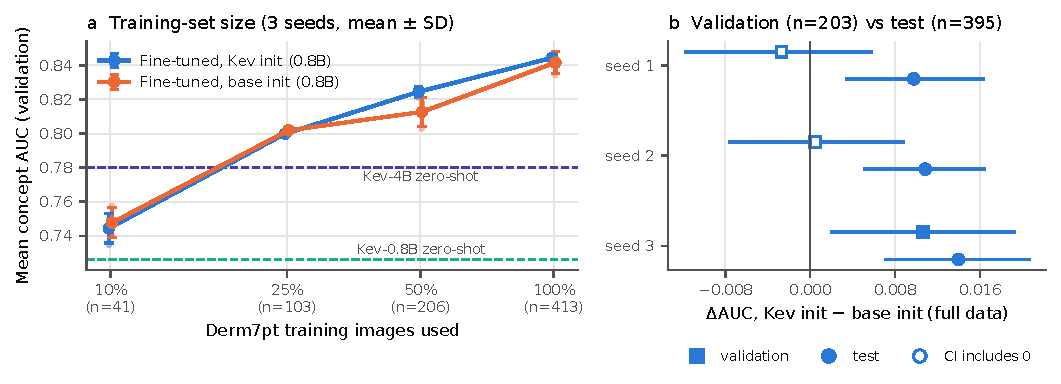
\includegraphics[width=\linewidth]{figs/fig4_kev_init.pdf}
\caption{Kev initialization and base initialization on Derm7pt. (a) Validation AUC by training-set size, as the mean $\pm$ standard deviation over three seeds; subsets of 10\% to 50\% use 300 optimizer steps on identical subsets per seed, and the full set uses six epochs. Dashed lines mark zero-shot references. (b) Paired \dauc{} per seed with the full training set, on validation (squares) and test (circles); hollow markers have intervals that include zero.}
\label{fig:kevinit}
\end{figure}

All fine-tuned models start from the same backbone and use the same data, augmentations, schedule and seeds; only the initialization of the adapters and the pointer head differs.

\paragraph{Accuracy.} On Derm7pt validation, Kev initialization did not meet the prespecified criterion, with mean AUCs of 0.8444 $\pm$ 0.0013 and 0.8415 $\pm$ 0.0064 and two of three intervals including zero (Figure~\ref{fig:kevinit}(b)). With 10\%, 25\% and 50\% of the training images, the mean differences were $-0.003$, $-0.002$ and $+0.012$ AUC, and none met the criterion (Figure~\ref{fig:kevinit}(a)). On the larger test set, all three seeds favor Kev initialization by 0.010 to 0.014 AUC, with a mean of 0.012 and every interval above zero. Because the validation comparison did not confirm it, we regard this gain as small and provisional. SLAKE shows the same direction, with differences of 0.002 to 0.008 AUC and one of three intervals above zero.

\paragraph{Training stability.} On VQA-RAD, one of three base-initialized runs collapsed to a test AUC of 0.659, whereas the three Kev-initialized runs reached 0.856 to 0.860. The standard deviation over seeds is 0.091 for base initialization and 0.002 for Kev initialization. Three seeds do not allow a failure rate to be estimated. The pattern is consistent with a benefit from starting the adapters and the pointer head from weights trained on typed decision tasks.

\subsection{Readout Comparison}
\begin{figure}[t]
\centering
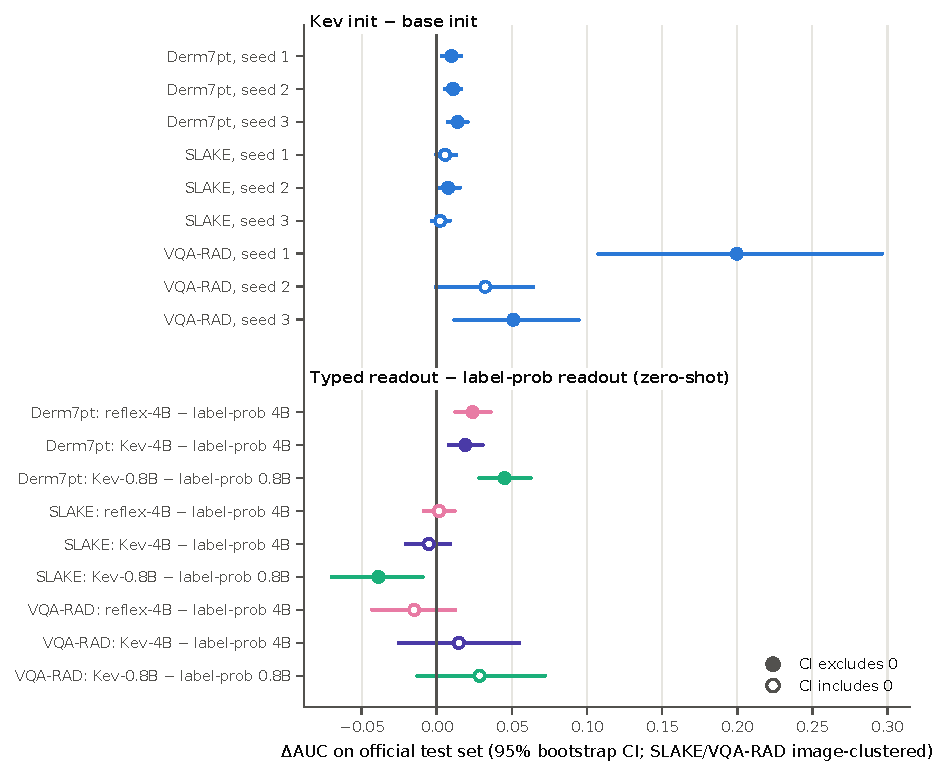
\includegraphics[width=0.86\linewidth]{figs/fig3_forest.pdf}
\caption{Prespecified paired comparisons on the official test sets. Markers are point estimates and bars are 95\% bootstrap intervals, resampled by image for SLAKE and VQA-RAD; filled markers have intervals that exclude zero. The upper block compares Kev initialization with base initialization per seed, and the lower block compares typed readouts with label readers of the same size in zero-shot use.}
\label{fig:forest}
\end{figure}

\paragraph{Dermoscopic criteria.} Figure~\ref{fig:forest} compares typed readouts with label readers of the same size. On Derm7pt, the typed readout achieves a higher mean AUC for all three pairs, by 0.024 for reflex, 0.019 for Kev-4B and 0.045 for Kev-0.8B, and every interval excludes zero. At 4B the advantage comes mainly from pigment network, where the label reader reaches 0.67 against 0.81 to 0.82 for the typed models. On the other three-way criteria the 4B results are mixed; for example, Kev-4B trails the label reader on streaks (0.75 against 0.80). At 0.8B, the typed readout leads on four of the five three-way criteria. A possible reason is that the label reader must bind option letters to their definitions~\citep{robinson2023mcq}.

\paragraph{Binary questions.} On binary radiology questions, the typed readout shows no advantage. On SLAKE, the 4B pairs differ by $+0.002$ [$-0.008$, $+0.012$] and $-0.005$ [$-0.021$, $+0.009$], and Kev-0.8B is lower than its label reader by 0.039 [$-0.070$, $-0.009$]. On VQA-RAD no pair differs significantly, although the intervals are wide; for Kev-0.8B the difference is $+0.029$ [$-0.013$, $+0.072$]. SLAKE is also close to saturation. On PubMedQA, the open 4B typed models have higher macro-F1 point estimates than the 4B label reader (0.566 and 0.582 against 0.546; not tested). There, the label reader reads the words yes, no and maybe directly, and its prior is skewed: it predicted ``maybe'' 139 times against 55 true cases.

\subsection{Calibration and Robustness Analysis}
\begin{figure}[t]
\centering
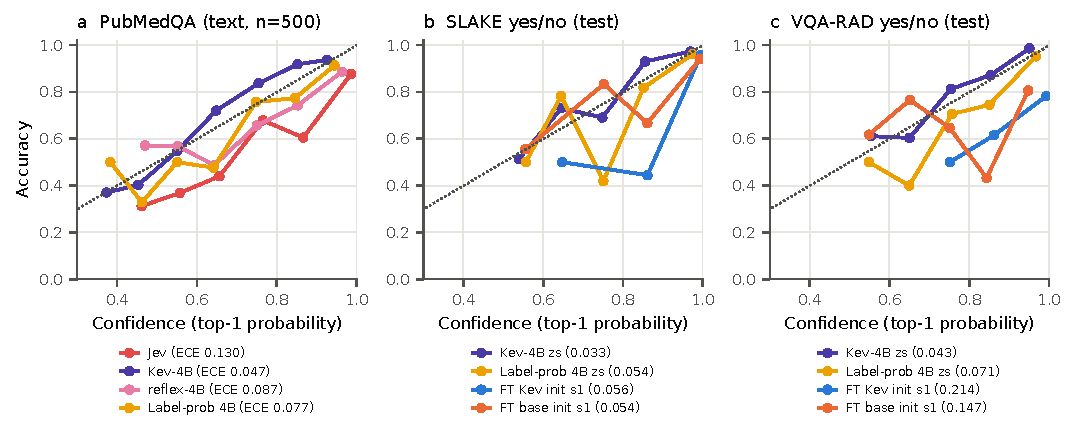
\includegraphics[width=\linewidth]{figs/fig5_reliability.pdf}
\caption{Reliability diagrams on the official test sets with 10 bins. Bins with fewer than five items are omitted, and legend values are ECE on the full set. Fine-tuned curves show seed 1; on VQA-RAD, base-initialization seed 1 is the collapsed run. (a) PubMedQA. (b) SLAKE. (c) VQA-RAD.}
\label{fig:rel}
\end{figure}

\paragraph{Calibration.} Figure~\ref{fig:rel} shows reliability diagrams. On binary radiology questions, the zero-shot typed models have low calibration error, with ECE of 0.023 to 0.033 on SLAKE and 0.043 to 0.054 on VQA-RAD for Kev-4B and reflex, against 0.054 and 0.071 for the 4B label reader (not tested). On Derm7pt, the ECE is 0.366 and 0.323 for the 4B and 0.8B label readers, 0.122 to 0.135 for the zero-shot typed models, and 0.047 to 0.066 for the fine-tuned models and linear probes. Fine-tuning does not guarantee calibration. On VQA-RAD, the Kev-initialized models have an ECE of 0.205 $\pm$ 0.010, with mean confidence of 0.96 to 0.97 against an accuracy of 0.76 to 0.77. This over-confidence is also present on the 24 test questions whose images were not seen during training. On PubMedQA, the hosted Jev is more accurate but less well calibrated than the open 4B-scale models (Table~\ref{tab:pubmedqa}), and its responses are not fully deterministic. Re-sending 100 identical requests changed two decisions and shifted probabilities by up to 0.10.

\begin{figure}[t]
\centering
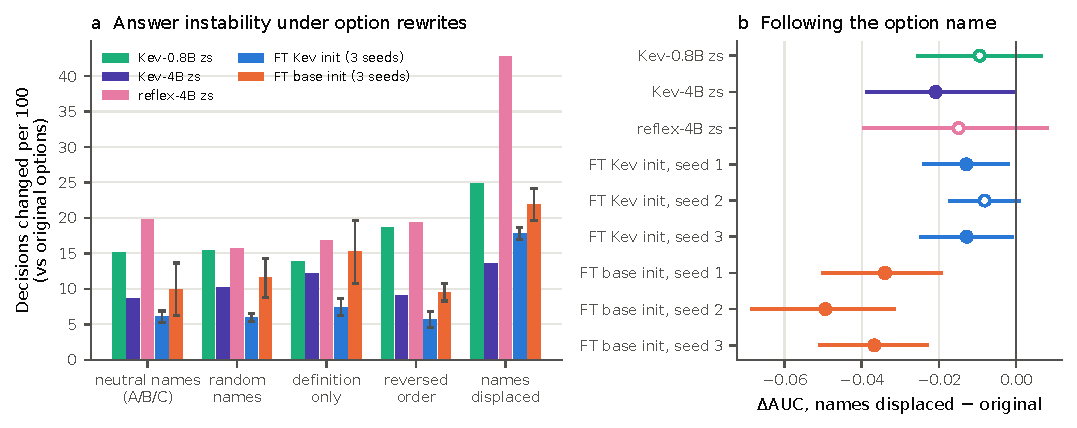
\includegraphics[width=\linewidth]{figs/fig6_option_names.pdf}
\caption{Sensitivity to option wording on Derm7pt validation for the five three-way criteria. (a) Decisions that change relative to the original options; fine-tuned bars give the mean $\pm$ standard deviation over three seeds. (b) AUC change when option names are displaced while definitions and ground truth remain fixed; hollow markers have intervals that include zero.}
\label{fig:names}
\end{figure}

\paragraph{Option names.} Following \citet{sun2026typesafe}, we rewrote the five three-way Derm7pt criteria on the validation split while keeping the ground truth tied to each option's definition (Figure~\ref{fig:names}). Displacing names cyclically across definitions, as in ``absent: irregular network with thickened lines'', lowered AUC for every model. For base initialization the drop was 0.034 to 0.049 AUC on every seed. For Kev initialization it was 0.008 to 0.013 AUC and significant for two of three seeds. The prespecified difference-in-differences, the Kev-initialized drop minus the base-initialized drop, was positive for all three seeds: $+0.021$ [$+0.009$, $+0.033$], $+0.041$ [$+0.027$, $+0.057$] and $+0.024$ [$+0.013$, $+0.034$]. Among zero-shot models the drop was significant only for Kev-4B, at $-0.021$ [$-0.039$, $-0.0002$]. These effects are much smaller than those reported for binary text workflows, where swapping option names lowered AUC from 0.94 to 0.23 for one open model and from 0.81 to 0.58 for Jev~\citep{sun2026typesafe}. Our manipulation is milder, and each of our options carries an explicit clinical definition.

\paragraph{Meaning-preserving rewrites.} Neutral names, random names, definitions without names, and reversed option order changed 4.4 to 20.3 of every 100 decisions. On average, Kev-initialized models changed 6.3 per 100 (range 4.4 to 8.8) and base-initialized models 11.6 (range 6.9 to 20.3), although this difference was not tested. reflex changed 19.3 decisions per 100 under reversed order despite averaging two option orders. Aggregate AUC moved by at most about 0.01 under these rewrites, but some shifts were significant, for example $+0.010$ for Kev-4B with neutral names. The borderline name-displacement effect for zero-shot Kev-4B is therefore only about twice this fluctuation.

\subsection{Criterion-Level Analysis}
Appendix Figure~\ref{fig:heat} reports test AUC per criterion. The salient blue-whitish veil is detected about as well without fine-tuning (AUC 0.89 to 0.92) as after fine-tuning (0.91). Subtle criteria benefit from training: for pigmentation and regression structures, zero-shot models reach 0.65 to 0.72 and fine-tuned models 0.81 to 0.84. The typed readout's advantage over label readers at 4B comes mainly from pigment network, whereas on pigmentation all zero-shot models remain near 0.65 to 0.70. Correct recognition of salient findings therefore coexists with weak recognition of subtle patterns in every zero-shot model.

%==========================================================================
\section{Conclusion}
%==========================================================================
We presented a typed visual readout that connects the native vision encoder of Qwen3.5 to an open typed decision model and returns a probability for each clinically defined option. Decision-oriented initialization extends this interface to medical fine-tuning by starting the adapters and the pointer head from weights trained on typed decision tasks.

Experiments across dermoscopy, radiology and biomedical text show where this interface adds value. The fine-tuned typed model achieves the highest mean AUC among the compared models on Derm7pt (0.851) and SLAKE (0.981), and the typed readout exceeds label probabilities on multi-option dermoscopic criteria but not on binary questions. Decision-oriented initialization reduced the effect of displaced option names in every seed, and none of its runs collapsed on VQA-RAD, whereas its accuracy gain was small and not confirmed on validation. On PubMedQA, the hosted Jev was more accurate but less well calibrated than open 4B-scale models. The evidence comes from four datasets, 0.8B-scale fine-tuning, validation-only option-name tests and a single query date for the hosted model, and it reports multiple paired comparisons without multiplicity correction. The calibration gap of the hosted model and the over-confidence of fine-tuned models on VQA-RAD identify two directions for further work: in-domain recalibration of typed readouts, and fine-tuning at larger scale with patient-level splits.

\section*{Data and Code Availability}
All datasets are public and were used under their original terms. Every number in this paper is computed from released prediction reports; means and standard deviations are derived by \texttt{derive\_numbers.py}, and test-set comparisons by \texttt{final\_test\_analysis.py}. Base repositories: Kev@5920c5f (Apache-2.0), reflex@231f896 (MIT), derm7pt@ce43687 and pubmedqa@1cbae8e (MIT).

\bibliographystyle{unsrtnat}
\bibliography{refs}

\newpage
\appendix
\section{Implementation Details}
\label{app:impl}
\paragraph{Interface checks.} Kev's own cached and uncached inference paths differ by up to $6.93\times10^{-4}$ in probability, and our interface matches the uncached path exactly. In a single-example gradient check, all 372 low-rank adapter tensors and the pointer head received non-zero gradients with Kev initialization; with base initialization, 186 of 372 did, because only the zero-initialized $B$ matrices receive gradient at the first step. The vision encoder received none. Outputs varied across images: $P(\text{veil})$ ranged from 0.143 to 0.823 over 20 Derm7pt images, although the raw decision states are highly similar across images (mean cosine 0.996, and $-0.009$ after centering).

\paragraph{Inputs per model.} reflex receives option names as keys with their definitions as values. Label readers do not receive the state description ``Medical image.'' used by Kev and reflex on SLAKE and VQA-RAD. Qwen-based local models receive $448\times448$ images, the BiomedCLIP probe uses its own $224\times224$ preprocessing, and reflex receives the original image. The probe regularization strength is chosen from $\{10^{-5},\dots,10\}$ by AUC.

\paragraph{Validation references.} The zero-shot Kev-0.8B value in Table~\ref{tab:val} and Figure~\ref{fig:kevinit}(a) is the epoch-0 evaluation of the fine-tuning pipeline, with the adapters warm-started from Kev and $T=1$. Low-data subsets are drawn once per seed and shared by both initializations, and bootstrap resamples in which a class is absent are redrawn.

\section{Additional Results}
\begin{figure}[h]
\centering
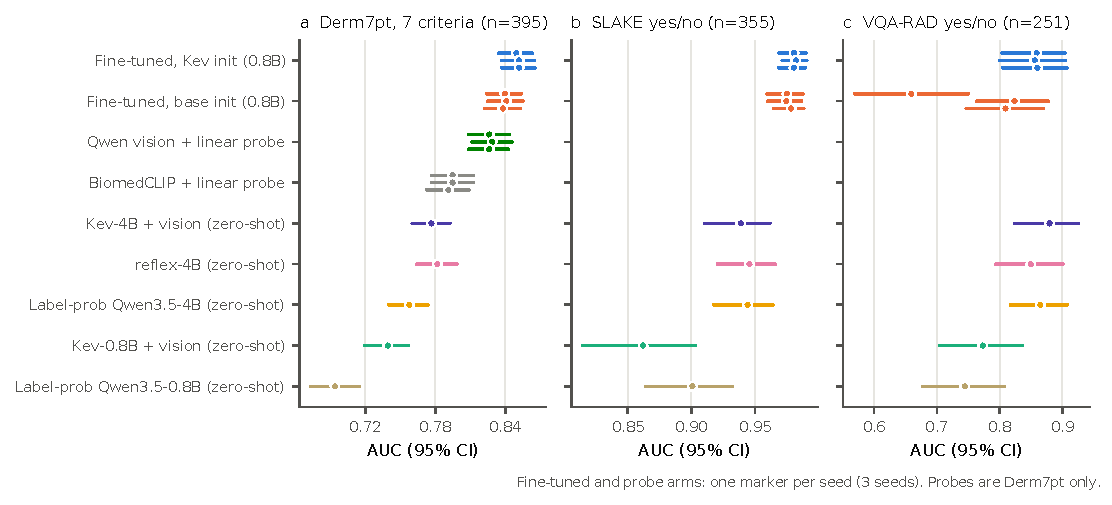
\includegraphics[width=\linewidth]{figs/fig2_landscape.pdf}
\caption{Test-set AUC with 95\% bootstrap intervals, resampled by image for SLAKE and VQA-RAD. Fine-tuned models and probes show one marker per seed.}
\label{fig:landscape}
\end{figure}

\begin{figure}[h]
\centering
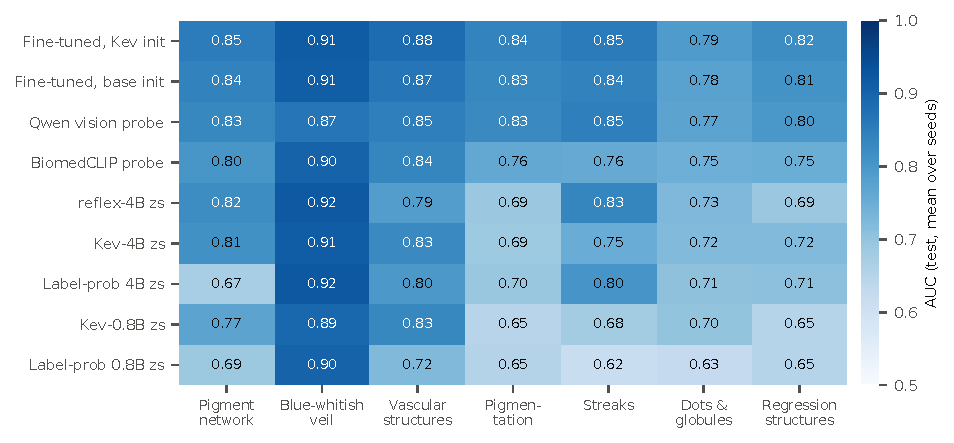
\includegraphics[width=0.9\linewidth]{figs/fig7_derm_heatmap.pdf}
\caption{Derm7pt test AUC per criterion, averaged over seeds where applicable.}
\label{fig:heat}
\end{figure}

\begin{figure}[h]
\centering
\begin{minipage}[t]{0.48\linewidth}\centering
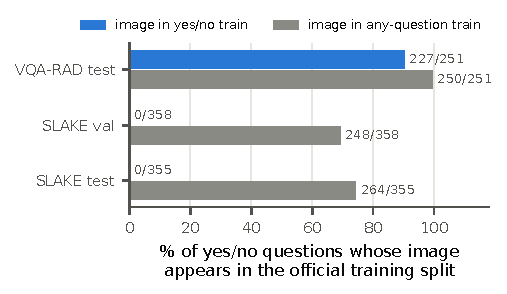
\includegraphics[width=\linewidth]{figs/fig8_leakage.pdf}
\caption{Share of official test and validation questions whose image file also occurs in the training split, relative to yes/no training questions and to all training questions.}
\label{fig:leak}
\end{minipage}\hfill
\begin{minipage}[t]{0.48\linewidth}\centering
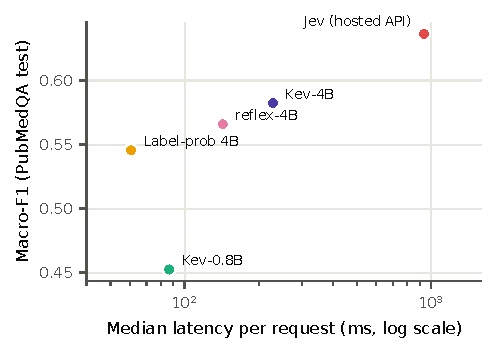
\includegraphics[width=\linewidth]{figs/fig9_pubmedqa_latency.pdf}
\caption{PubMedQA macro-F1 against median latency per request on a logarithmic scale. Jev latency includes the network round trip.}
\label{fig:lat}
\end{minipage}
\end{figure}

\begin{table}[h]
\centering
\caption{Derm7pt validation results. Trained and probe rows give the mean $\pm$ standard deviation over three seeds; zero-shot rows are single deterministic runs.}
\label{tab:val}
\small
\begin{tabular}{lcc}
\toprule
Setting & Kev initialization & Base initialization \\
\midrule
10\% of training lesions (41) & 0.744 $\pm$ 0.009 & 0.748 $\pm$ 0.009 \\
25\% (103) & 0.800 $\pm$ 0.002 & 0.802 $\pm$ 0.001 \\
50\% (206) & 0.824 $\pm$ 0.003 & 0.813 $\pm$ 0.008 \\
100\% (413; six epochs) & 0.844 $\pm$ 0.001 & 0.842 $\pm$ 0.006 \\
\midrule
BiomedCLIP with linear probe & \multicolumn{2}{c}{0.798 $\pm$ 0.003} \\
Qwen encoder with linear probe & \multicolumn{2}{c}{0.816 $\pm$ 0.002} \\
Kev-0.8B (zero-shot) & \multicolumn{2}{c}{0.726} \\
Kev-4B (zero-shot) & \multicolumn{2}{c}{0.780} \\
\bottomrule
\end{tabular}
\end{table}

\section{Protocol Notes}
\label{app:posthoc}
\paragraph{Evaluation checklist.} Relative to the TDM evaluation checklist~\citep{audit2026tdm}, the protocol includes a label-probability baseline (4B on all datasets, 0.8B on the image datasets), task-specific baselines, option-order and option-name tests, repeated hosted requests, versioned models and repositories, paired bootstrap intervals, calibration measurements and prespecified decision rules. It does not include a generative cascade baseline, accuracy at fixed confidence thresholds, or latency with response caching.

\paragraph{Scope of the evidence.} The hosted Jev accepts only text, so the image results concern open Jev-style models. The Kev and label-reader contrasts at 0.8B and 4B also differ in pretraining, because Kev uses Base checkpoints and the label readers use instruction-tuned ones. Derm7pt provides no patient identifiers, so splits could be checked at the lesion level only, and image overlap was measured on byte-identical files. The paper reports about 78 paired comparisons without multiplicity correction, several near the interval boundary. Bootstrap intervals treat trained weights as fixed and do not capture seed variance, which three seeds cannot estimate.

\paragraph{Post-hoc choices.} The BiomedCLIP probe's regularization grid was extended to $10^{-5}$ and $10^{-4}$ after the first selection fell on the grid edge; the selected value and the result did not change. Two Derm7pt runs had stored only their best-validation checkpoint and were retrained with identical seeds to obtain the final-epoch weights, which reproduced the original final-epoch validation AUC (0.8453 and 0.8456). Image-disjoint re-splits of SLAKE and VQA-RAD were prepared but are not used. The low-data study and the option-name test were designed after the full-data comparison on Derm7pt validation, with decision rules written before they were run. The three-seed option-name comparison was added after an internal review found that the first version used one seed per initialization; the single-seed results are reproduced exactly within it.

\end{document}
